%
% $Id: fase.tex 14 2014-02-04 22:36:30Z nicb $
%
% p.76 cap.4 n.7
%
\svnInfo $Id: fase.tex 14 2014-02-04 22:36:30Z nicb $

\section{La risposta in fase\label{sec:phase}}

Riconsideriamo ancora una volta il filtro che abbiamo analizzato in
Cap.\ref{chap:fir} Sez.\vref{sec:simple fir} (eq.\ref{eqn:fir semplice}):

		\begin{equation}\label{eqn:fir semplice 2}
						y_t = x_t + a_1 x_{t-\tau}
			\end{equation}

la cui risposta in frequenza \`e una funzione della frequenza $\omega$

	\begin{equation}\label{eqn:fir semplice frqresp}
	       H ( \omega ) = 1 + a_1 e^{-i \omega}
	\end{equation}

Questa risposta complessa in frequenza avr\`a quindi una magnitudine e un
angolo per ciascun $\omega$. Cio\`e l'eq.\ref{eqn:fir semplice frqresp} pu\`o
essere riscritta come 

	\begin{equation}\label{eqn:fir semplice frqresp 2}
	       1 + a_1 e^{-i \omega} = |H ( \omega )| e^{i \Theta ( \omega )}
	\end{equation}

Se il segnale in ingresso fosse un fasore complesso $x = e^{i \omega t}$,
il fasore in uscita $y$ sarebbe il prodotto di questo ingresso moltiplicato
questa funzione di trasferimento

	\begin{equation}\label{eqn:fs output}
		y_t = |H ( \omega )|e^{i (\omega t + \Theta ( \omega ) )}
	\end{equation}

il che significa che l'uscita \`e una copia dell'ingresso ritardata in fase di
un angolo $\Theta ( \omega )$ e riscalata in ampiezza di $| H ( \omega )|$.

Per capire quanto valga il ritardo di fase possiamo usare la funzione
\emph{arcotangente}. Riscrivendo l'eq.\ref{eqn:fir semplice frqresp} come $1 +
a_1 cos \omega - i a_1 sin \omega$, avremo

  \begin{equation}\label{eqn:risp in fase}
			\begin{array}{r c l}
							\Theta ( \omega ) & = & arctan \left [ \frac{\mathpzc{Immag} H ( \omega )}{\mathpzc{Reale} H ( \omega )} \right ]\\
							                  & = & arctan \left [ \frac{- a_1 sin \omega}{1 + a_1 cos \omega} \right ]\\
			\end{array}
	\end{equation}

Quando $a_1 = 1$ l'espressione contenuta in eq.\ref{eqn:risp in fase} si
semplifica. Riscrivendo la funzione di trasferimento di eq.\ref{eqn:fir semplice frqresp}
con $a_1 = 1$:

	\begin{equation}\label{eqn:fir semplice frqresp 3}
			H ( \omega ) = 1 + e^{-i \omega} = e^{-i \omega / 2} \left [ e^{i \omega / 2} + e^{-i \omega / 2} \right ]
	\end{equation}

Ricordiamo che la formula di Eulero $e^{i \alpha} = cos \alpha + i sin
\alpha$, e che quindi

	\begin{equation}\label{eqn:remember eulero}
			\begin{array}{r c l}
							cos \alpha & = & \frac{e^{i \alpha} + e^{-i \alpha}}{2}\\
							sin \alpha & = & \frac{e^{i \alpha} - e^{-i \alpha}}{2i}\\
							e^{i \alpha} + e^{-i \alpha} & = & 2 cos \alpha\\
							e^{i \omega / 2 } + e^{-i \omega / 2} & = & 2 cos \omega / 2\\
			\end{array}
	\end{equation}

	allora l'eq.\ref{eqn:fir semplice frqresp 3} si semplifica in

  \begin{equation}\label{eqn:fir semplice frqresp 3 result}
		H (\omega) =  e^{-i \omega / 2} 2 cos (\omega / 2)\\
	\end{equation}

Confrontando l'eq.\ref{eqn:fir semplice frqresp 2} con la \ref{eqn:fir semplice frqresp 3 result},
$2 cos (\omega / 2)$ \`e la magnitudine della risposta (reale) $|H ( \omega )|$,
mentre l'esponenziale complesso $e^{-i \omega / 2}$ \`e la risposta in fase
e rappresenta un ritardo di fase di un angolo $- \omega / 2$.
Quindi, se l'ingresso \`e il fasore $e^{i \omega t}$, l'uscita del filtro
sar\`a il fasore

	\begin{equation}\label{eqn:fir output}
			2 cos ( \omega / 2 ) e^{i \omega (t - 1 / 2)}
	\end{equation}

il che equivale a dire che l'effetto del filtro sulla fase del segnale \`e
quello di ritardarlo esattamente di un tempo equivalente alla met\`a della
frequenza di campionamento, \emph{indipendentemente dalla frequenza} $\omega$
\emph{del fasore in ingresso}.

Questo \`e un caso speciale di una caratteristica importante dei filtri FIR:
se i coefficienti di un filtro FIR sono simmetrici intorno al proprio centro
(in questo caso i coefficienti sono $\{ 1, 1 \}$, la risposta in fase \`e
proporzionale ad $\omega$, trattandosi quindi di un ritardo di tempo fisso per
tutte le frequenze. Il filtro si dice quindi \emph{a fase lineare}, ossia non
introduce distorsioni nella risposta in fase.

La fig.\vref{fig: fase 3} riporta la risposta in frequenza e la risposta in
fase del filtro FIR

\begin{equation}\label{eqn: fir 3}
	H ( z ) = 0.5 - 0.8 z^{-1} + 0.5 z^{-2}
\end{equation}
\begin{figure}[htb]
	\begin{center}
	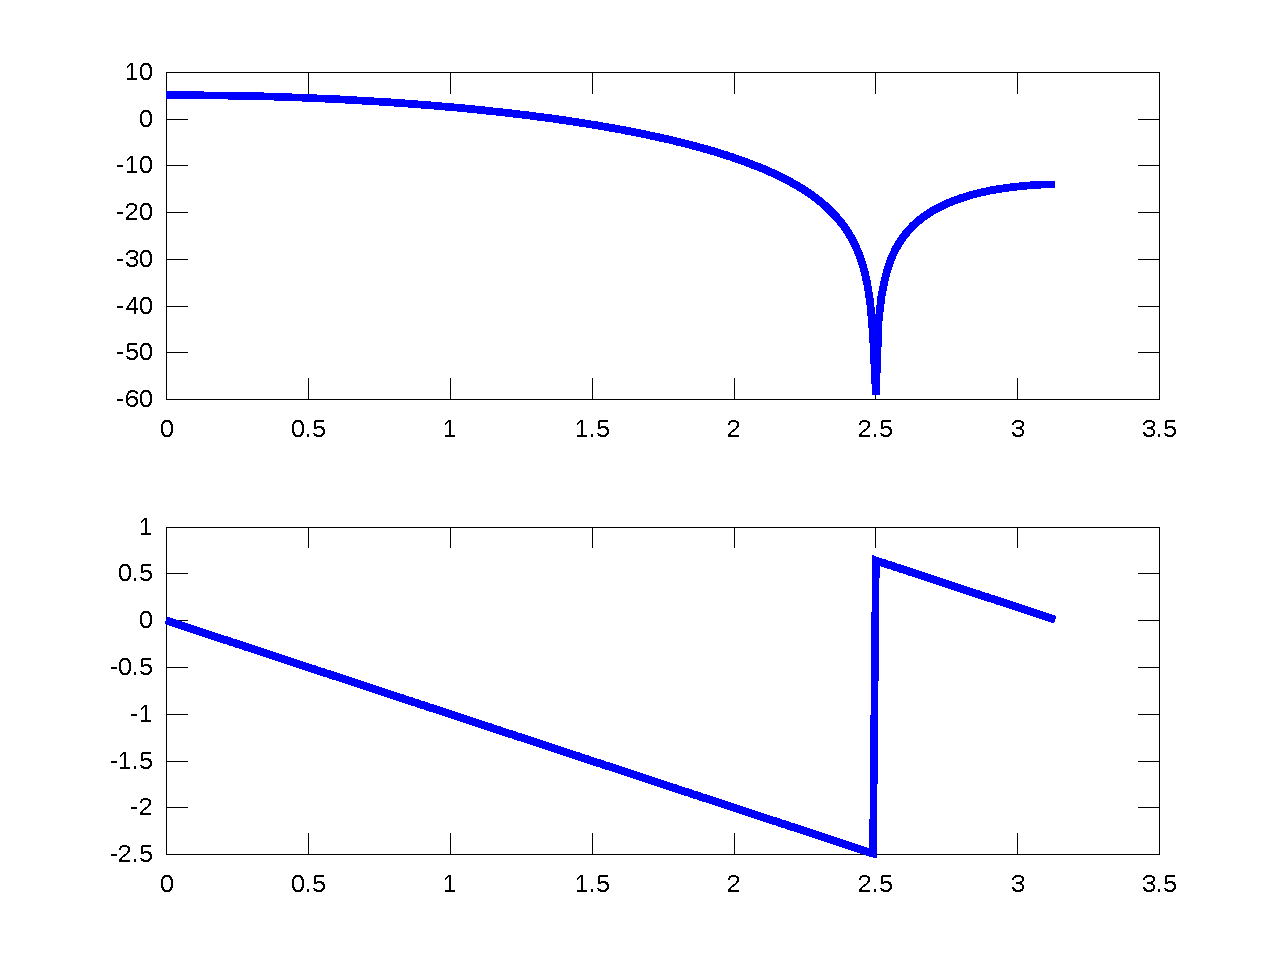
\includegraphics[width=0.9\textwidth]{\plotdir/fase_3}
	\caption{Risposta in frequenza e in fase del filtro la cui funzione di
	trasferimento \`e riportata in eq.\ref{eqn: fir 3}\label{fig: fase 3}}
	\end{center}
\end{figure}

Come si pu\`o notare, un numero dispari di coefficienti genera una risposta in
fase lineare.

Lo script {\tt octave} che genera questa figura \`e riportato qui:

\verbatiminput{\plotdir/fase_3.m}
